\let\negmedspace\undefined
\let\negthickspace\undefined
\documentclass[journal,12pt,onecolumn]{IEEEtran}
\usepackage{cite}
\usepackage{amsmath,amssymb,amsfonts,amsthm}
\usepackage{algorithmic}
\usepackage{graphicx}
\graphicspath{{./figs/}}
\usepackage{textcomp}
\usepackage{xcolor}
\usepackage{txfonts}
\usepackage{listings}
\usepackage{enumitem}
\usepackage{mathtools}
\usepackage{gensymb}
\usepackage{comment}
\usepackage{caption}
\usepackage[breaklinks=true]{hyperref}
\usepackage{tkz-euclide} 
\usepackage{listings}
\usepackage{gvv}                                        
%\def\inputGnumericTable{}                                 
\usepackage[latin1]{inputenc}     
\usepackage{xparse}
\usepackage{color}                                            
\usepackage{array}                                            
\usepackage{longtable}                                       
\usepackage{calc}                                             
\usepackage{multirow}
\usepackage{multicol}
\usepackage{hhline}                                           
\usepackage{ifthen}                                           
\usepackage{lscape}
\usepackage{tabularx}
\usepackage{array}
\usepackage{float}
\newtheorem{theorem}{Theorem}[section]
\newtheorem{problem}{Problem}
\newtheorem{proposition}{Proposition}[section]
\newtheorem{lemma}{Lemma}[section]
\newtheorem{corollary}[theorem]{Corollary}
\newtheorem{example}{Example}[section]
\newtheorem{definition}[problem]{Definition}
\newcommand{\BEQA}{\begin{eqnarray}}
\newcommand{\EEQA}{\end{eqnarray}}
\newcommand{\define}{\stackrel{\triangle}{=}}
\theoremstyle{remark}
\newtheorem{rem}{Remark}

\begin{document}

\title{
ASSIGNMENT 4: GATE 2022 \\
IN: INSTRUMENTATION ENGINEERING}
\author{EE25BTECH11062 - Vivek K Kumar}
\maketitle
\renewcommand{\thefigure}{\theenumi}
\renewcommand{\thetable}{\theenumi}

\begin{enumerate}
\item Inhaling the smoke from a burning \underline{\hspace{2cm}} could \underline{\hspace{2cm}} you quickly.

\hfill{\brak{\text{GATE IN 2022}}}
\begin{enumerate}
\item tire/tier
\item tire/tyre
\item tyre/tire
\item tyre/tier
\end{enumerate}

\item A sphere of radius $r$ cm is packed in a box of cubical shape. What should be the minimum volume \brak{\text{in } cm^3} of the box that can enclose the sphere?

\hfill{\brak{\text{GATE IN 2022}}}
\begin{enumerate}
\item $\frac{r^3}{8}$
\item $r^3$
\item $2r^3$
\item $8r^3$
\end{enumerate}

\item Pipes P and Q can fill a storage tank in full with water in $10$ and $6$ minutes, respectively. Pipe R draws the water out from the storage tank at a rate of $34$ litres per minute. P, Q and R operate at a constant rate. If it takes one hour to completely empty a full storage tank with all the pipes operating simultaneously, what is the capacity of the storage tank \brak{\text{in litres}}?

\hfill{\brak{\text{GATE IN 2022}}}
\begin{enumerate}
\item $26.8$
\item $60.0$
\item $120.0$
\item $127.5$
\end{enumerate}

\item Six persons P, Q, R, S, T and U are sitting around a circular table facing the center not necessarily in the same order. Consider the following statements:
\begin{itemize}
\item P sits next to S and T.
\item Q sits diametrically opposite to P.
\item The shortest distance between S and R is equal to the shortest distance between T and U.
\end{itemize}
Based on the above statements, Q is a neighbor of

\hfill{\brak{\text{GATE IN 2022}}}
\begin{enumerate}
\item U and S
\item R and T
\item R and U
\item P and S
\end{enumerate}

\item A building has several rooms and doors as shown in the top view of the building given below. The doors are closed initially. What is the minimum number of doors that need to be opened in order to go from the point P to the point Q?

\hfill{\brak{\text{GATE IN 2022}}}
\begin{figure}[H]
\includegraphics[width = 0.5\columnwidth]{q5}
\caption*{}
\label{fig:q5}
\end{figure}
\begin{enumerate}
\item $4$
\item $3$
\item $2$
\item $1$
\end{enumerate}

\item Rice, a versatile and inexpensive source of carbohydrate, is a critical component of diet worldwide. Climate change, causing extreme weather, poses a threat to sustained availability of rice. Scientists are working on developing Green Super Rice (GSR), which is resilient under extreme weather conditions yet gives higher yields sustainably. Which one of the following is the CORRECT logical inference based on the information given in the above passage?

\hfill{\brak{\text{GATE IN 2022}}}
\begin{enumerate}
\item GSR is an alternative to regular rice, but it grows only in an extreme weather
\item GSR may be used in future in response to adverse effects of climate change
\item GSR grows in an extreme weather, but the quantity of produce is lesser than regular rice
\item Regular rice will continue to provide good yields even in extreme weather
\end{enumerate}

\item A game consists of spinning an arrow around a stationary disk as shown below. When the arrow comes to rest, there are eight equally likely outcomes. It could come to rest in any one of the sectors numbered $1$, $2$, $3$, $4$, $5$, $6$, $7$ or $8$ as shown. Two such disks are used in a game where their arrows are independently spun. What is the probability that the sum of the numbers on the resulting sectors upon spinning the two disks is equal to $8$ after the arrows come to rest?

\hfill{\brak{\text{GATE IN 2022}}}
\begin{figure}[H]
\includegraphics[width = 0.5\columnwidth]{q7}
\caption*{}
\label{fig:q7}
\end{figure}
\begin{enumerate}
\item $\frac{1}{16}$
\item $\frac{5}{64}$
\item $\frac{3}{32}$
\item $\frac{7}{64}$
\end{enumerate}

\item Consider the following inequalities.
\begin{align*}
\brak{\text{i}} \qquad 3p-q&<4\\
\brak{\text{ii}}\qquad 3q-p&<12
\end{align*}
Which one of the following expressions below satisfies the above two inequalities?

\hfill{\brak{\text{GATE IN 2022}}}
\begin{enumerate}
\item $p+q<8$
\item $p+q=8$
\item $8\le p+q<16$
\item $p+q\ge16$
\end{enumerate}

\item Given below are three statements and four conclusions drawn based on the statements.
\begin{itemize}
\item Statement 1: Some engineers are writers.
\item Statement 2: No writer is an actor.
\item Statement 3: All actors are engineers.
\end{itemize}
\begin{itemize}
\item Conclusion I: Some writers are engineers.
\item Conclusion II: All engineers are actors.
\item Conclusion III: No actor is a writer.
\item Conclusion IV: Some actors are writers.
\end{itemize}
Which one of the following options can be logically inferred?

\hfill{\brak{\text{GATE IN 2022}}}
\begin{enumerate}
\item Only conclusion I is correct
\item Only conclusion II and conclusion III are correct
\item Only conclusion I and conclusion III are correct
\item Either conclusion III or conclusion IV is correct
\end{enumerate}

\item Which one of the following sets of pieces can be assembled to form a square with a single round hole near the center? Pieces cannot overlap.

\hfill{\brak{\text{GATE IN 2022}}}
\begin{figure}[H]
\begin{enumerate}
\item \includegraphics[width = 0.4\columnwidth]{q10a} 
\item \includegraphics[width = 0.4\columnwidth]{q10b}
\item \includegraphics[width = 0.4\columnwidth]{q10c}
\item \includegraphics[width = 0.4\columnwidth]{q10d}
\end{enumerate}
\caption*{}
\label{fig:q10}
\end{figure}

\item The input $x\brak{t}$ to a system is related to its output $y\brak{t}$ as
\begin{align*}
\frac{dy\brak{t}}{dt}+y\brak{t}=3x\brak{t-3}u\brak{t-3}
\end{align*}
Here $u\brak{t}$ represents a unit-step function. The transfer function of this system is

\hfill{\brak{\text{GATE IN 2022}}}
\begin{enumerate}
\item \begin{align*} \frac{e^{-3s}}{s+3} \end{align*}
\item \begin{align*} \frac{3e^{-3s}}{s+1} \end{align*}
\item \begin{align*} \frac{3e^{-\brak{s/3}}}{s+1} \end{align*}
\item \begin{align*} \frac{e^{-\brak{s/3}}}{s+3} \end{align*}
\end{enumerate}

\item A pneumatic nozzle-flapper system is conventionally used to convert

\hfill{\brak{\text{GATE IN 2022}}}
\begin{enumerate}
\item Small changes in flapper's velocity to large changes in output temperature
\item Small changes in flapper's displacement to large changes in output temperature
\item Small changes in flapper's velocity to large changes in output pressure
\item Small changes in flapper's displacement to large changes in output pressure
\end{enumerate}

\item A periodic function $f\brak{x}$, with period $2$, is defined as
\begin{align*}
f\brak{x} = \begin{cases} -1 - x & -1 \le x < 0 \\ 1 - x & 0 < x \le 1 \end{cases}
\end{align*}
The Fourier series of this function contains \underline{\hspace{2cm}}

\hfill{\brak{\text{GATE IN 2022}}}
\begin{enumerate}
\item Both $\cos \brak{n\pi x}$ and $\sin \brak{n\pi x}$ where $n = 1, 2, 3, \ldots$
\item Only $\sin \brak{n\pi x}$ where $n = 1, 2, 3, \ldots$
\item Only $\cos \brak{n\pi x}$ where $n = 1, 2, 3, \ldots$
\item Only $\cos \brak{2n\pi x}$ where $n = 1, 2, 3, \ldots$
\end{enumerate}

\item The output of a system $y\brak{t}$ is related to its input $x\brak{t}$ according to the relation
\begin{align*}
y\brak{t} = x\brak{t} \sin\brak{2\pi t}
\end{align*}
This system is \underline{\hspace{2cm}}

\hfill{\brak{\text{GATE IN 2022}}}
\begin{enumerate}
\item Linear and time-variant
\item Non-linear and time-invariant
\item Linear and time-invariant
\item Non-linear and time-variant
\end{enumerate}

\item A unity-gain negative-feedback control system has a loop-gain $L\brak{s}$ given by
\begin{align*}
L\brak{s} = \frac{6}{s\brak{s-5}}
\end{align*}
The closed-loop system is \underline{\hspace{2cm}}

\hfill{\brak{\text{GATE IN 2022}}}
\begin{enumerate}
\item Causal and stable
\item Causal and unstable
\item Non-causal and stable
\item Non-causal and unstable
\end{enumerate}

\item A sinusoidal carrier wave with amplitude $A_c$ and frequency $f_c$ is amplitude modulated with a message signal $m\brak{t}$ having frequency $0 < f_m \ll f_c$ to generate the modulated wave $s\brak{t}$ given by
\begin{align*}
s\brak{t} = A_c\brak{1 + m\brak{t}}\cos \brak{2\pi f_c t} 
\end{align*}
The message signal that can be retrieved completely using envelope detection is \underline{\hspace{2cm}}

\hfill{\brak{\text{GATE IN 2022}}}
\begin{enumerate}
\item $m\brak{t} = 0.5 \cos\brak{2\pi f_m t}$
\item $m\brak{t} = 1.5 \sin\brak{2\pi f_m t}$
\item $m\brak{t} = 2 \sin\brak{4\pi f_m t}$
\item $m\brak{t} = 2 \cos \brak{4\pi f_m t}$
\end{enumerate}

\item A Hall sensor is based on the principle of \underline{\hspace{2cm}}

\hfill{\brak{\text{GATE IN 2022}}}
\begin{enumerate}
\item Photoelectric effect
\item Seebeck effect
\item Piezoelectric effect
\item Lorentz force
\end{enumerate}

\item A signal $x\brak{t}$ is band-limited between $100$ Hz and $200$ Hz. A signal $y\brak{t}$ is related to $x\brak{t}$ as follows:
\begin{align*}
y\brak{t} = x\brak{2t - 5} 
\end{align*}
The statement that is always true is \underline{\hspace{2cm}}

\hfill{\brak{\text{GATE IN 2022}}}
\begin{enumerate}
\item $y\brak{t}$ is band-limited between $50$ Hz and $100$ Hz
\item $y\brak{t}$ is band-limited between $100$ Hz and $200$ Hz
\item $y\brak{t}$ is band-limited between $200$ Hz and $400$ Hz
\item $y\brak{t}$ is not band-limited
\end{enumerate}

\item The figure shows a Chromel-Alumel thermocouple, where the junction A is held at temperature $T_A$, and a thermal emf $E_1$ is measured using an ideal voltmeter between the open ends B1 and B2, both held at temperature $T_B$. Two identical copper wires are introduced between B1-C1 and B2-C2 as shown in the figure. When C1 and C2 are held at temperature $T_C$, the voltmeter reads a thermal emf $E_2$. Then, \underline{\hspace{2cm}}

\hfill{\brak{\text{GATE IN 2022}}}
\begin{figure}[H]
\includegraphics[width = 0.75\columnwidth]{q19}
\caption*{}
\label{fig:q19}
\end{figure}
\begin{enumerate}
\item $E_1 < E_2$
\item $E_1 > E_2$
\item $E_1 = 2E_2$
\item $E_1 = E_2$
\end{enumerate}

\item The resistance of a pure copper wire of length $10$ cm and diameter $1$ mm is to be measured. The most suitable method from amongst the choices given below is \underline{\hspace{2cm}}

\hfill{\brak{\text{GATE IN 2022}}}
\begin{enumerate}
\item Two wire method
\item Three wire method
\item Four wire method
\item Ellipsometry
\end{enumerate}

\item The logic block shown has an output $F$ given by \underline{\hspace{2cm}}

\hfill{\brak{\text{GATE IN 2022}}}
\begin{figure}[H]
\includegraphics[width = 0.5\columnwidth]{q21}
\caption*{}
\label{fig:q21}
\end{figure}
\begin{enumerate}
\item $A + B$
\item $A \cdot \overline{B}$
\item $\overline{A + B}$
\item $\overline{B}$
\end{enumerate}

\item In which of the following bridge\brak{s} is the balancing condition frequency-independent?

\hfill{\brak{\text{GATE IN 2022}}}
\begin{enumerate}
\item Maxwell bridge
\item Wien bridge
\item Schering bridge
\item Wheatstone bridge
\end{enumerate}

\item The output F of the digital circuit shown can be written in the form\brak{s} \underline{\hspace{2cm}}

\hfill{\brak{\text{GATE IN 2022}}}
\begin{figure}[H]
\includegraphics[width = 0.7\columnwidth]{q23}
\caption*{}
\label{fig:q23}
\end{figure}
\begin{enumerate}
\item $\overline{\overline{A \cdot B}}$
\item $\overline{A} + \overline{B}$
\item $\overline{A+B}$
\item $\overline{A} \cdot \overline{B}$
\end{enumerate}

\item Given $M = \myvec{ 2 & 3 & 7 \\ 6 & 4 & 7 \\ 4 & 6 & 14 }$, which of the following statement\brak{s} is/are correct?

\hfill{\brak{\text{GATE IN 2022}}}
\begin{enumerate}
\item The rank of $M$ is $2$
\item The rank of $M$ is $3$
\item The rows of $M$ are linearly independent
\item The determinant of $M$ is $0$
\end{enumerate}

\item An analog-to-digital converter with resolution $0.01$ V converts analog signals between $0$ V to $+10$ V to an unsigned binary output. The minimum number of bits \brak{\text{in integer}} in the output is \underline{\hspace{2cm}}

\hfill{\brak{\text{GATE IN 2022}}}

\item Consider $24$ voice signals being transmitted without latency using time-division multiplexing. If each signal is sampled at $12$ kHz and represented by an $8$-bit word, the bit-duration \brak{\text{in microseconds}} is \underline{\hspace{2cm}} \brak{\text{round off to two decimal places}}

\hfill{\brak{\text{GATE IN 2022}}}

\item A photodiode is made of a semiconductor with a bandgap of $1.42$ eV. Given that Planck's constant is $6.626 \times 10^{-34}$ Js, the speed of light in vacuum is $3 \times 10^8$ m/s, and $1$ eV = $1.6 \times 10^{-19}$ J, the cut-off wavelength \brak{\text{in nanometers}} of the photodiode is \underline{\hspace{2cm}} \brak{\text{round off to one decimal place}}

\hfill{\brak{\text{GATE IN 2022}}}

\item The global minimum of $x^3 e^{-|x|}$ for $x \in \brak{-\infty, \infty}$ occurs at $x = \underline{\hspace{2cm}}$ \brak{\text{round off to one decimal place}}

\hfill{\brak{\text{GATE IN 2022}}}

\item A $440$ V, $8$ kW, $4$-pole, $50$ Hz, star-connected induction motor has a full load slip of $0.04$. The rotor speed \brak{\text{in rpm}} at full load is \underline{\hspace{2cm}} \brak{\text{round off to one decimal place}}

\hfill{\brak{\text{GATE IN 2022}}}

\item The transfer function of a system is: $\frac{\brak{s+1}\brak{s+3}}{\brak{s+5}\brak{s+7}\brak{s+9}}$. In the state-space representation of the system, the minimum number of state variables \brak{\text{in integer}} necessary is \underline{\hspace{2cm}}

\hfill{\brak{\text{GATE IN 2022}}}

\item A Zener diode is used as a $4$ V voltage regulator in the circuit shown. Given that the diode requires a minimum current of $4$ mA for voltage regulation, the maximum current \brak{\text{in milliamperes}} permitted to flow through the load $R_L$ is \underline{\hspace{2cm}} \brak{\text{round off to one decimal place}}

\hfill{\brak{\text{GATE IN 2022}}}
\begin{figure}[H]
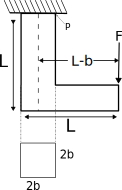
\includegraphics[width = 0.5\columnwidth]{q31}
\caption*{}
\label{fig:q31}
\end{figure}

\item A bag contains six red balls and four blue balls. If three balls are drawn in succession without replacement, the probability that the second and third balls drawn are red is \underline{\hspace{2cm}} \brak{\text{round off to two decimal places}}

\hfill{\brak{\text{GATE IN 2022}}}

\item In the bandpass filter circuit shown, $R_0 = 50$ \ohm, $L_0 = 1$ mH, $C_0 = 10$ nF. The Q factor of the filter is \underline{\hspace{2cm}} \brak{\text{round off to two decimal places}}

\hfill{\brak{\text{GATE IN 2022}}}
\begin{figure}[H]
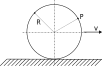
\includegraphics[width = 0.6\columnwidth]{q33}
\caption*{}
\label{fig:q33}
\end{figure}

\item The Newton-Raphson method is applied to determine the solution of $f\brak{x} = 0$ where $f\brak{x} = x - \cos \brak{x}$. If the initial guess of the solution is $x_0 = 0$, the value of the next approximation $x_1$ is \underline{\hspace{2cm}} \brak{\text{round off to two decimal places}}

\hfill{\brak{\text{GATE IN 2022}}}

\item An OPAMP has a gain of $10^4$, an input impedance of $10$ M\ohm \ and an output impedance of $100$ \ohm. The OPAMP is used in unity-gain feedback configuration in a voltage buffer circuit. The closed-loop output impedance of the OPAMP \brak{\text{in milliohms}} in the circuit is \underline{\hspace{2cm}} \brak{\text{round off to one decimal place}}

\hfill{\brak{\text{GATE IN 2022}}}

\item A signal $V_{in}\brak{t}$ shown is applied from $t = 0$ ms to $t = 6$ ms to the circuit shown. Given the initial voltage across the capacitor is $0.3$ V, and that the diode is ideal, the open circuit voltage $V_{out}\brak{t}$ at $t = 5$ ms is \underline{\hspace{2cm}}

\hfill{\brak{\text{GATE IN 2022}}}
\begin{figure}[H]
\includegraphics[width = 0.7\columnwidth]{q36}
\caption*{}
\label{fig:q36}
\end{figure}
\begin{enumerate}
\item $0.3$ V
\item $0.6$ V
\item $0.7$ V
\item $1.0$ V
\end{enumerate}

\item The signal flow graph of a system is shown. The expression for $Y\brak{s}/X\brak{s}$ is \underline{\hspace{2cm}}

\hfill{\brak{\text{GATE IN 2022}}}
\begin{figure}[H]
\includegraphics[width = 0.7\columnwidth]{q37}
\caption*{}
\label{fig:q37}
\end{figure}
\begin{enumerate}
\item 
\begin{align*}
    \frac{2G_1\brak{s}G_2\brak{s} + 2G_1\brak{s}G_3\brak{s}}{1+G_2\brak{s}+G_3\brak{s}}
\end{align*}
\item 
\begin{align*}
\frac{2 + G_1\brak{s} + G_3\brak{s} + G_2\brak{s}}{1+G_2\brak{s}}
\end{align*}
\item 
\begin{align*}
\frac{G_1\brak{s} + G_3\brak{s} - G_2\brak{s}}{2 + G_2\brak{s}} 
\end{align*}
\item 
\begin{align*}
\frac{2G_1\brak{s}G_2\brak{s} + 2G_1\brak{s}G_3\brak{s} - G_1\brak{s}}{1+G_2\brak{s}+G_3\brak{s}} 
\end{align*}
\end{enumerate}

\item Consider the transfer function $H_c\brak{s} = \frac{1}{\brak{s+1}\brak{s+3}}$. Bilinear transformation with a sampling period of $0.1$ s is employed to obtain the discrete-time transfer function $H_d\brak{z}$. Then $H_d\brak{z}$ is \underline{\hspace{2cm}}

\hfill{\brak{\text{GATE IN 2022}}}
\begin{enumerate}
\item \begin{align*}\frac{\brak{1 + z^{-1}}^2}{\brak{19 - 21z^{-1}}\brak{23 - 17z^{-1}}}\end{align*}
\item \begin{align*}\frac{\brak{1 - z^{-1}}^2}{\brak{21 - 19z^{-1}}\brak{17 - 23z^{-1}}}\end{align*}
\item \begin{align*}\frac{\brak{1 + z^{-1}}^2}{\brak{21 - 19z^{-1}}\brak{23 - 17z^{-1}}}\end{align*}
\item \begin{align*}\frac{\brak{1 + z^{-1}}^2}{\brak{21 - 19z^{-1}}\brak{17 - 23z^{-1}}}\end{align*}
\end{enumerate}

\item A car is moving collinearly with a laser beam emitted by a transceiver. A laser pulse emitted at $t = 0$ s is received back by the transceiver $100$ ns \brak{\text{nanoseconds}} later after reflection from the car. A second pulse emitted at $t = 0.1$ s is received back $90$ ns later. Given the speed of light is $3 \times 10^8$ m/s, the average speed of the car in this interval is \underline{\hspace{2cm}}

\hfill{\brak{\text{GATE IN 2022}}}
\begin{enumerate}
\item $54$ kmph, moving towards the transceiver
\item $108$ kmph, moving towards the transceiver
\item $54$ kmph, moving away from the transceiver
\item $108$ kmph, moving away from the transceiver
\end{enumerate}

\item The signal $x\brak{t} = \brak{t - 1}^2 u\brak{t - 1}$, where $u\brak{t}$ is the unit-step function, has the Laplace transform $X\brak{s}$. The value of $X\brak{1}$ is \underline{\hspace{2cm}}

\hfill{\brak{\text{GATE IN 2022}}}
\begin{enumerate}
\item $\frac{1}{e}$
\item $\frac{2}{e}$
\item $2e$
\item $e^2$
\end{enumerate}

\item A proportional-integral-derivative \brak{PID} controller is employed to stably control a plant with transfer function $P\brak{s} = \frac{1}{\brak{s+1}\brak{s+2}}$. Now, the proportional gain is increased by a factor of $2$, the integral gain is increased by a factor of $3$, and the derivative gain is left unchanged. Given that the closed-loop system continues to remain stable with the new gains, the steady-state error in tracking a ramp reference signal \underline{\hspace{2cm}}

\hfill{\brak{\text{GATE IN 2022}}}
\begin{enumerate}
\item Remains unchanged
\item Decreases by a factor of $2$
\item Decreases by a factor of $3$
\item Decreases by a factor of $5$
\end{enumerate}

\item A resistor ladder digital-to-analog converter \brak{DAC} receives a digital input that results in the circuit having the state as shown in the figure. For this digital input, the Thevenin voltage, $V_{th}$, and Thevenin resistance, $R_{th}$, as seen at the output node are \underline{\hspace{2cm}}

\hfill{\brak{\text{GATE IN 2022}}}
\begin{figure}[H]
\includegraphics[width = 0.5\columnwidth]{q42}
\caption*{}
\label{fig:q42}
\end{figure}
\begin{enumerate}
\item $V_{th} = 0.5$ V, $R_{th}= 1$ k\ohm
\item $V_{th}= 0.5$ V, $R_{th}= 2$ k\ohm
\item $V_{th}= 1$ V, $R_{th}= 1$ k\ohm
\item $V_{th}= 1$ V, $R_{th}= 2$ k\ohm
\end{enumerate}

\item The Nyquist plot of a stable open-loop system $G\brak{j\omega}$ is plotted in the frequency range $0 \le \omega < \infty$ as shown. It is found to intersect a unit circle with center at the origin at the point $P = -0.77 - 0.64j$. The points $Q$ and $R$ lie on $G\brak{j\omega}$ and assume values $Q = 14.40 + 0.00j$ and $R = -0.21 + 0.00j$. The phase margin \brak{PM} and the gain margin \brak{GM} of the system are \underline{\hspace{2cm}}

\hfill{\brak{\text{GATE IN 2022}}}
\begin{figure}[H]
\includegraphics[width = 0.5\columnwidth]{q43}
\caption*{}
\label{fig:q43}
\end{figure}
\begin{enumerate}
\item PM = $39.7\degree$ and GM = $4.76$
\item PM = $39.7\degree$ and GM = $0.07$
\item PM = $-39.7\degree$ and GM = $4.76$
\item PM = $-39.7\degree$ and GM = $0.07$
\end{enumerate}

\item In the small signal circuit shown, the enhancement mode n-channel MOSFET is biased in saturation with transconductance $g_m$. If channel length modulation is ignored, the small signal impedance looking into the node P is given by \underline{\hspace{2cm}}

\hfill{\brak{\text{GATE IN 2022}}}
\begin{figure}[H]
\includegraphics[width = 0.5\columnwidth]{q44}
\caption*{}
\label{fig:q44}
\end{figure}
\begin{enumerate}
\item \begin{align*}R_S||R_L|| g_m^{-1}\end{align*}
\item \begin{align*}R_S||g_m^{-1}\end{align*}
\item \begin{align*}\brak{R_S + R_L}||g_m^{-1}\end{align*}
\item \begin{align*}\frac{R_L g_m}{1 + R_S g_m\brak{R_L||g_m^{-1}}}\end{align*}
\end{enumerate}

\item Consider the differential equation $\frac{dy}{dx} + y \ln\brak{y} = 0$. If $y\brak{0} = e$, then $y\brak{1}$ is \underline{\hspace{2cm}}

\hfill{\brak{\text{GATE IN 2022}}}
\begin{enumerate}
\item $e^e$
\item $e^{-e}$
\item $e^{\brak{1/e}}$
\item $e^{-\brak{1/e}}$
\end{enumerate}



\item The digital circuit shown \underline{\hspace{2cm}}

\hfill{\brak{\text{GATE IN 2022}}}
\begin{figure}[H]
\includegraphics[width = 0.55\columnwidth]{q46}
\caption*{}
\label{fig:q46}
\end{figure}
\begin{enumerate}
\item is a divide-by-$5$ counter
\item is a divide-by-$7$ counter
\item is a divide-by-$8$ counter
\item does not function as a counter due to disjoint cycles of states
\end{enumerate}

\item In the small signal circuit shown, the enhancement mode n-channel MOSFET is biased in saturation with a transconductance $g_m$. A small signal low-frequency voltage $v_d$ injected at the supply terminal results in a small signal voltage fluctuation $v_o$ at the output. If the channel length modulation of the MOSFET is ignored, the small signal gain $v_o/v_d$ is given by \underline{\hspace{2cm}}

\hfill{\brak{\text{GATE IN 2022}}}
\begin{figure}[H]
\includegraphics[width = 0.3\columnwidth]{q47}
\caption*{}
\label{fig:q47}
\end{figure}
\begin{enumerate}
\item \begin{align*}\frac{-g_m R_0}{1 + g_m R_0}\end{align*}
\item \begin{align*}\brak{g_m R_0 + 1}^{-1}\end{align*}
\item \begin{align*}\frac{-g_m R_0}{1 + 2g_m R_0}\end{align*}
\item \begin{align*}\brak{\frac{g_m R_0}{2} + \frac{3}{2}}^{-1}\end{align*}
\end{enumerate}

\item $A = a_1 a_0$ and $B = b_1 b_0$ are two $2$-bit unsigned binary numbers. If $F\brak{a_1, a_0, b_1, b_0}$ is a Boolean function such that $F = 1$ only when $A > B$, and $F = 0$ otherwise, then $F$ can be minimized to the form \underline{\hspace{2cm}}

\hfill{\brak{\text{GATE IN 2022}}}
\begin{enumerate}
\item $a_1 \overline{b}_1 + a_1 a_0 \overline{b}_0$
\item $a_1 \overline{b}_1 + a_1 a_0 \overline{b}_0 + a_0 \overline{b}_0 \overline{b}_1$
\item $a_1 a_0 \overline{b}_0 + a_0 \overline{b}_0 \overline{b}_1$
\item $a_1 \overline{b}_1 + a_1 a_0 \overline{b}_0 + a_0 \overline{b}_0 b_1$
\end{enumerate}

\item The matrix $A = \myvec{4 & 3 \\ 9 & -2}$ has eigenvalues $-5$ and $7$. The eigenvector\brak{s} is/are \underline{\hspace{2cm}}

\hfill{\brak{\text{GATE IN 2022}}}
\begin{enumerate}
\item \myvec{ 1 \\ 1 }
\item \myvec{ 3 \\ 4 }
\item \myvec{ 2 \\ -6 }
\item \myvec{ 2 \\ 8 }
\end{enumerate}

\item For the complex number $z = \frac{a+jb}{a-jb}$, where $a>0$ and $b>0$. Which of the following statement\brak{s} is/are true?

\hfill{\brak{\text{GATE IN 2022}}}
\begin{enumerate}
\item The phase is $2 \tan^{-1} \frac{b}{a}$
\item The phase is $\tan^{-1} \frac{2b}{a}$
\item The magnitude is $1$
\item The magnitude is $\sqrt{\frac{a^2+b^2}{a^2-b^2}}$
\end{enumerate}

\item Monochromatic light of wavelength $532$ nm is used to measure the absorption coefficient of a material in a UV-Visible Spectrophotometer. The measured light intensity after transmission through a $1$ cm thick sample of the material is $0.414$ mW/cm$^2$. For a sample of thickness $2$ cm, the measured light intensity is $0.186$ mW/cm$^2$. The absorption coefficient \brak{\text{in } cm^{-1}} of the material is \underline{\hspace{2cm}} \brak{\text{round off to two decimal places}}

\hfill{\brak{\text{GATE IN 2022}}}

\item In the circuit shown, the load is driven by a sinusoidal ac voltage source $V_1 = 100 \angle 0\degree$ V at $50$ Hz. Given $R_1 = 20$ \ohm, $C_1 = \brak{\frac{1000}{\pi}}$ \textmu F, $L_1 = \brak{\frac{20}{\pi}}$ mH and $R_2 = 4$ \ohm, the power factor is \underline{\hspace{2cm}} \brak{\text{round off to one decimal place}}

\begin{figure}[H]
    \centering
    \includegraphics[width=0.5\columnwidth]{q52}
    \caption*{}
    \label{fig:q52}
\end{figure}

\hfill{\brak{\text{GATE IN 2022}}}

\item In a unity-gain feedback control system, the plant $P\brak{s} = \frac{0.001}{s\brak{2s+1}\brak{0.01s+1}}$ is controlled by a lag compensator $C\brak{s} = \frac{s+10}{s+0.1}$. The slope \brak{\text{in dB/decade}} of the asymptotic Bode magnitude plot of the loop gain at $\omega = 3$ rad/s is \underline{\hspace{2cm}} \brak{\text{in integer}}

\hfill{\brak{\text{GATE IN 2022}}}



\item Given Circuit A with currents $I_1$ and $I_2$ as shown, the current $I_3$ in Circuit B \brak{\text{in amperes}}, is \underline{\hspace{2cm}}\brak{\text{round off to one decimal place}}

\hfill{\brak{\text{GATE IN 2022}}}

\begin{figure}[H]
\includegraphics[width = 0.6\columnwidth]{q54}
\caption*{}
\label{fig:q54}
\end{figure}

\item In the balanced three-phase circuit shown, $C_0 = 8.2$ \textmu F and the line-to-line r.m.s. voltage is $440$ V at $50$ Hz. The reading on the wattmeter \brak{\text{in watts}} is \underline{\hspace{2cm}} \brak{\text{round off to two decimal places}}

\hfill{\brak{\text{GATE IN 2022}}}
\begin{figure}[H]
\includegraphics[width = 0.5\columnwidth]{q55}
\caption*{}
\label{fig:q55}
\end{figure}

\item The circuit shown is driven by a sinusoidal input voltage, $V_{in}$, resulting in the output voltage, $V_{out}$. The frequency \brak{\text{in kilohertz}} at which the voltage gain is $0$ dB is \underline{\hspace{2cm}} \brak{\text{round off to two decimal places}}

\hfill{\brak{\text{GATE IN 2022}}}
\begin{figure}[H]
\includegraphics[width = 0.7\columnwidth]{q56}
\caption*{}
\label{fig:q56}
\end{figure}

\item A conducting semi-circular loop of radius $R = 0.1$ m, with its diameter centered at the origin, rotates in the x-y plane about the origin with a constant angular velocity, $\omega = 20$ rad/s, as shown. A magnetic field of magnitude $B = 2$ T and normal to x-y plane exists in the region $x \ge 0$ as shown. If the loop has a resistance of $2$ \ohm, and negligible inductance, the peak-to-peak current \brak{\text{in milliamperes}} in the loop is \underline{\hspace{2cm}} \brak{\text{round off to one decimal place}}

\hfill{\brak{\text{GATE IN 2022}}}
\begin{figure}[H]
\includegraphics[width = 0.5\columnwidth]{q57}
\caption*{}
\label{fig:q57}
\end{figure}

\item In the circuit shown, $R_1=100$ k\ohm \ and $R_2=1$ k\ohm. If the base-to-emitter voltage of the npn BJT is $0.7$ V and the collector-to-emitter voltage is $5.2$ V, the $\beta$ \brak{\text{current gain}} of the BJT is \underline{\hspace{2cm}} \brak{\text{round off to two decimal places}}

\hfill{\brak{\text{GATE IN 2022}}}
\begin{figure}[H]
\includegraphics[width = 0.5\columnwidth]{q58}
\caption*{}
\label{fig:q58}
\end{figure}

\item A capacitor is constructed using two concentric spheres and air as the dielectric medium \brak{\text{permittivity of air } = 8.854 \times 10^{-12} \text{ F/m}}. The radii of the inner and outer spheres are $a = 10$ cm and $b=15$ cm, respectively. The capacitance \brak{\text{in picofarads}} is \underline{\hspace{2cm}} \brak{\text{round off to } 2 \text{ decimal places}}

\hfill{\brak{\text{GATE IN 2022}}}

\item A $1$ kHz sine-wave generator having an internal resistance of $50$ \ohm \ generates an open-circuit voltage of $10$ Vp-p. When a capacitor is connected across the output terminals, the voltage drops to $8$ Vp-p. The capacitance of the capacitor \brak{\text{in microfarads}} is \underline{\hspace{2cm}} \brak{\text{round off to two decimal places}}

\hfill{\brak{\text{GATE IN 2022}}}

\item Consider the function $f\brak{z} = \frac{1}{\brak{z+1}\brak{z+2}\brak{z+3}}$. The residue of $f\brak{z}$ at $z = -1$, is \underline{\hspace{2cm}}

\hfill{\brak{\text{GATE IN 2022}}}

\item In the circuit shown, the capacitance $C_0 = 10$ \textmu F and inductance $L_0 = 1$ mH and the diode is ideal. The capacitor is initially charged to $10$ V and the current in the inductor is initially zero. If the switch is closed at $t = 0$ s, the voltage $V_c\brak{t}$ \brak{\text{in volts}} across the capacitor at $t = 0.5$ s is \underline{\hspace{2cm}} \brak{\text{round off to one decimal place}}

\hfill{\brak{\text{GATE IN 2022}}}
\begin{figure}[H]
\includegraphics[width = 0.5\columnwidth]{q62}
\caption*{}
\label{fig:q62}
\end{figure}

\item The bridge shown is balanced when $R_1= 100$ \ohm, $R_2 = 210$ \ohm, $C_2 = 2.9$ \textmu F, and $R_4 = 50$ \ohm. The $2$ kHz sine-wave generator supplies a voltage of $10$ Vp-p. The value of $L_3$ \brak{\text{in millihenry}} is \underline{\hspace{2cm}} \brak{\text{round off to two decimal places}}

\hfill{\brak{\text{GATE IN 2022}}}
\begin{figure}[H]
\includegraphics[width = 0.5\columnwidth]{q63}
\caption*{}
\label{fig:q63}
\end{figure}

\item In the circuit shown, the switch is initially closed. It is opened at $t = 0$ s and remains open thereafter. The time \brak{\text{in milliseconds}} at which the output voltage $V_{out}$ becomes LOW is \underline{\hspace{2cm}} \brak{\text{round off to three decimal places}}

\hfill{\brak{\text{GATE IN 2022}}}
\begin{figure}[H]
\includegraphics[width = 0.6\columnwidth]{q64}
\caption*{}
\label{fig:q64}
\end{figure}

\item In the Wheatstone bridge circuit shown, $R_1 = 1.5$ k\ohm \ and $R_2 = R_3 = R_4 = 1$ k\ohm. The switch is initially open and the voltage between the points C and D is $V_{CD}$. Upon closing the switch at $t = 0$, the resistance in the arm AD changes by an amount $\delta R_1$, and the voltage between C and D changes by $\delta V_{CD}$. The sensitivity of the bridge \brak{\text{in volt/kiloohm}}, defined as $\abs{\frac{\delta V_{CD}}{\delta R_1}}$, is \underline{\hspace{2cm}} \brak{\text{round off to two decimal places}}

\hfill{\brak{\text{GATE IN 2022}}}
\begin{figure}[H]
\includegraphics[width = 0.6\columnwidth]{q65}
\caption*{}
\label{fig:q65}
\end{figure}
\end{enumerate}
\end{document}
